\chapter{Heaps}
\chaplabel{heaps}

In this chapter we discuss two implementations of the extremely useful
priority #Queue# data structure.  The first is an implementation based
on arrays.  It is very fast, and is the basis of one of the fastest
known sorting algorithms, namely heapsort.  The second implementation is
based on binary trees and is more flexible.  In particular, it supports
a #meld(h)# operation that allows the priority queue to absorb the
elements of a second priority queue #h#.

\section{#BinaryHeap#: An Implicit Binary Tree}
\seclabel{binaryheap}

Our first implementation of a (priority) #Queue# is based on a technique
that is over 400 years old.  Eytzinger's method allows us to represent a
complete binary tree as an array.  This is done by laying out the nodes
of the tree in breadth-first order (see \secref{bintree:traversal}) in
the array.  In this way, the root is stored at position 0, the root's
left child is stored at position 1, the root's right child at position 2,
the left child of the left child of the root is stored at position 3,
and so on. See \figref{eytzinger}.

\begin{figure}
  \begin{center}
    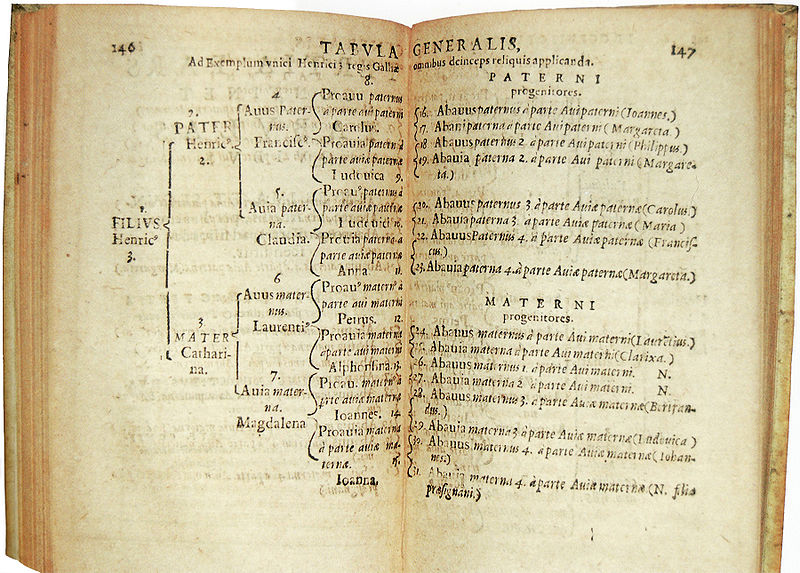
\includegraphics{figs/eytzinger}
  \end{center}
  \caption{Eytzinger's method represents a complete binary tree as an array.}
  \figlabel{eytzinger}
\end{figure}

If we do this for a large enough tree, some patterns emerge.  The left
child of the node at index #i# is at index $#left(i)#=2#i#+1$ and the
right child of the node at index #i# is at index $#right(i)#=2#i#+2$.
The parent of the node at index #i# is at index $#parent(i)#=(#i#-1)/2$.
\javaimport{ods/BinaryHeap.left(i).right(i).parent(i)}

A #BinaryHeap# uses this technique to implicitly represent a complete
binary tree in which the elements are \emph{heap-ordered}:  The value
stored at any index #i# is not smaller than the value stored at index
#parent(i)#, with the exception of the root value, $#i#=0$.  It follows
that the smallest value in the priority #Queue# is therefore stored at
position 0 (the root).

In a #BinaryHeap#, the #n# elements are stored in an array #a#:
\javaimport{ods/BinaryHeap.a.n}

Implementing the #add(x)# operation is fairly straightforward.
As with all array-based structures, we first check if #a# is full
(because $#a.length#=#n#$) and, if so, we grow #a#.  Next, we place #x#
at location #a[n]# and increment #n#.  At this point, all that remains is
to ensure that we maintain the heap property.  We do this by repeatedly
swapping #x# with its parent until #x# is no smaller than its parent.  See \figref{heap-insert}.
\javaimport{ods/BinaryHeap.add(x).bubbleUp(i)}

\begin{figure}
  \begin{center}
    \includegraphics{figs/heap-insert-1} \\
    \includegraphics{figs/heap-insert-2} \\
    \includegraphics{figs/heap-insert-3} \\
    \includegraphics{figs/heap-insert-4} \\
  \end{center}
  \caption{Inserting the value 6 into a #BinaryHeap#.}
  \figlabel{heap-insert}
\end{figure}

Implementing the #remove()# operation, which removes the smallest value
from the heap, is a little trickier.  We know where the smallest value is
(at the root), but we need to replace it after we remove it and ensure
that we maintain the heap property.

The easiest way to do this is to replace the root with the value #a[n]#
and decrement #n#.  Unfortunately, the new element now at the root is
probably not the smallest element, so it needs to be moved downwards.
We do this by repeatedly comparing this element to its two children.
If it is the smallest of the three then we are done.  Otherwise, we swap
this element with the smallest of its two children and continue.
\javaimport{ods/BinaryHeap.remove().trickleDown(i)}

\begin{figure}
  \begin{center}
    \includegraphics{figs/heap-remove-1} \\
    \includegraphics{figs/heap-remove-2} \\
    \includegraphics{figs/heap-remove-3} \\
    \includegraphics{figs/heap-remove-4} \\
  \end{center}
  \caption{Removing the minimum value, 4, from a #BinaryHeap#.}
  \figlabel{heap-remove}
\end{figure}



As with other array-based structures we will ignore the time spent in
calls to #resize()# since these can be accounted for with the amortization
argument from \lemref{arraystack-amortized}.  The running-times of
both #add(x)# and #remove()# then depend on the height of the (implicit)
binary tree.  However, this is a \emph{complete} binary tree;  every level
except the last has the maximum possible number of nodes.  Therefore,
if the height of this tree is $h$, then it has at least $2^h$ nodes.
Stated another way
\[
  #n# \ge 2^h \enspace .
\]  
Taking logarithms on both sides of this equation gives
\[
   h \le \log #n# \enspace .
\]
Therefore, both the #add(x)# and #remove()# operation run in $O(\log #n#)$ time.

\subsection{Summary}

The following theorem summarizes the performance of a #BinaryHeap#:

\begin{thm}\thmlabel{binaryheap}
  A #BinaryHeap# implements the (priority) #Queue# interface.  Ignoring
  the cost of calls to #resize()#, a #BinaryHeap# supports the operations
  #add(x)# and #remove()# in $O(\log #n#)$ time per operation.

  Furthermore, beginning with an empty #BinaryHeap#, any sequence of $m$
  #add(x)# and #remove()# operations results in a total of $O(m)$
  time spent during all calls to #resize()#.
\end{thm}

\section{#MeldableHeap#: A Randomized Meldable Heap}
\seclabel{meldableheap}

In this section, we describe the #MeldableHeap#, a priority #Queue#
implementation in which the underlying structure is also a heap-ordered
binary tree.  However, unlike a #BinaryHeap# in which the underlying
binary tree is completely defined by the number of elements, there
are no restrictions on the shape of the binary tree that underlies
a #MeldableHeap#; anything goes.

The #add(x)# and #remove()# operations in a #MeldableHeap# are
implemented in terms of the #merge(h1,h2)# operation.  This operation
takes two heap nodes #h1# and #h2# and merges them, returning a heap
node that is the root of a heap that contains all elements in the subtree
rooted at #h1# and all elements in the subtree rooted at #h2#.

The nice thing about a #merge(h1,h2)# operation is that it can be defined
recursively.  If either of #h1# or #h2# is #null#, then we
are merging with an empty set, so we return #h2# or #h1#, respectively.
Otherwise, assume $#h1.x# < #h2.x#$, since otherwise we can reverse the
roles of #h1# and #h2#.  Then we know that the root of the merged heap
will contain #h1.x# and we can recursively merge #h2# with #h1.left#
or #h1.right#, as we wish.  This is where randomization comes in, and we
toss a coin to decide whether to merge #h2# with #h1.left# or #h1.right#:
\javaimport{ods/MeldableHeap.merge(h1,h2)}

In the next section, we show that #merge(h1,h2)# runs in $O(\log #n#)$
expected time, where #n# is the total number of elements in #h1# and #h2#.

With access to a #merge(h1,h2)# operation, the #add(x)# operation is easy.  We create a new node #u# containing #x# and then merge #u# with the root of our heap:
\javaimport{ods/MeldableHeap.add(x)}
This takes $O(\log (#n#+1)) = O(\log #n#)$ expected time.

The #remove()# operation is similarly easy.  The node we want to remove
is the root, so we just merge its two children and make the result the root:
\javaimport{ods/MeldableHeap.remove()}
Again, this takes $O(\log #n#)$ expected time.

Additionally, a #MeldableHeap# can implement many other operations in
$O(\log #n#)$ expected time, including:
\begin{itemize}
\item #remove(u)# remove the node #u# (and its key #u.x#) from the heap.
\item #absorb(h)# add all the elements of the #MeldableHeap# #h# to this heap, emptying #h# in the process.
\end{itemize}
Each of these operations can be implemented using a constant number of
#merge(h1,h2)# operations that each take $O(\log #n#)$ time.

\subsection{Analysis of #merge(h1,h2)#}

The analysis of #merge(h1,h2)# is based on the analysis of a random walk
in a binary tree.  A \emph{random walk} in a binary tree is a walk that
starts at the root of the tree.  At each step in the walk, a coin is
tossed and the walk proceeds to the left or right child of the current
node depending on the result of this coin toss.  The walk ends when it
falls off the tree (the current node becomes #null#).

The following lemma is somewhat remarkable because it does not depend
at all on the shape of the binary tree:

\begin{lem}
The expected length of a random walk in a binary tree with #n# nodes is at most #\log (n+1)#.
\end{lem}

\begin{proof}
The proof is by induction on #n#. In the base case, $#n#=0$ and the walk
has length $0=\log (#n#+1)$.  Suppose now that the result is true for
all non-negative integers $#n#'< #n#$

Let $#n#_1$ denote the size of the root's left subtree, so that
$#n#_2=#n#-#n#_1-1$ is the size of the root's right subtree.  Starting at
the root, the walk takes one step and then continues in a subtree of size
$#n#_1$ or continues in a subtree of size $#n#_2$.  By our inductive
hypothesis, the expected length of the walk is then
\[
    \E[W] = 1 + \frac{1}{2}\log (#n#_1+1) + \frac{1}{2}\log (#n#_2+1)  \enspace , 
\] 
since each of $#n#_1$ and $#n#_2$ are less than $#n#$.
To maximize this, over the choice of $#n#_1\in[0,#n#-1]$, we
take the derivative and obtain
\[
    (\E[W])' = \frac{1}{2}(c/#n#_1 - c/(#n#-#n#_1-1)) \enspace , 
\]
which is equal to 0 when $#n#_1 = (#n#-1)/2$.  We can establish that
this is a maximum fairly easily, so the expected number of steps taken by the random walk is 
\begin{align*}
    \E[W] 
    & = 1 + \frac{1}{2}\log (#n#_1+1) + \frac{1}{2}\log (#n#_2+1) \\
   & \le  1 + \log ((#n#-1)/2+1) \\
   & =  1 + \log ((#n#+1)/2) \\
   & =  \log (#n#+1)  \enspace . \qedhere 
\end{align*}
\end{proof}

With this result on random walks, we can now easily prove that the
running time of the #merge(h1,h2)# operation is $O(\log #n#)$.

\begin{lem}
  If #h1# and #h2# are the roots of two heaps containing $#n#_1$
  and $#n#_2$ nodes, respectively, then the expected running time of
  #merge(h1,h2)# is at most $O(\log #n#)$, where $#n#=#n#_1+#n#_2$.
\end{lem}

\begin{proof}
  Each step of the merge algorithm takes one step of a random walk,
  either in the heap rooted at #h1# or the heap rooted at #h2#, depending
  on whether $#h1.x# < #h2.x#$ or not.  The algorithm terminates when
  either of these two random walks falls out of its corresponding tree
  (when $#h1#=#null#$ or $#h2#=#null#$).  Therefore, the expected number
  of steps performed by the merge algorithm is at most
  \[
     \log (#n#_1+1) + \log (#n#_2+1) \le 2\log #n# \enspace . \qedhere
  \]
\end{proof}

\subsection{Summary}

The following theorem summarizes the performance of a #MeldableHeap#:

\begin{thm}\thmlabel{meldableheap}
  A #MeldableHeap# implements the (priority) #Queue# interface.
  A #MeldableHeap# supports the operations #add(x)# and #remove()#
  in $O(\log #n#)$ expected time per operation.
\end{thm}

\section{Discussion and Exercises}

The implicit representation of a complete binary tree as an array,
or list, seems to have been first proposed by Eytzinger \cite{e1590},
as a representation for pedigree family trees.  The #BinaryHeap# data
structure described here was first introduced by Williams \cite{w64}.

The randomized #MeldableHeap# data structure described here appears
to have first been proposed by Gambin and Malinowski \cite{gm98}.
Other meldable heap implementations exist, including leftist heaps
\cite[Section~5.3.2]{c72,k97v3}, binomial heaps \cite{v78}, Fibonacci
heaps \cite{ft87}, pairing heaps \cite{fsst86}, and skew heaps
\cite{st83}, although none of these are as simple as the #MeldableHeap#
structure described here.

Some of the above structures also support a #decreaseKey(u,y)# operation
in which the value stored at node #u# is decreased to #y#.  (It is a
pre-condition that $#y#\le#u.x#$.)  This operation can be implemented
in $O(\log #n#)$ time in most of the above structures by removing node
#u# and adding  #y#.  However, some of these structures can implement
#decreaseKey(u,y)# more efficiently.  In particular, #decreaseKey(u,y)#
takes $O(1)$ amortized time in Fibonacci heaps and $O(\log\log #n#)$
amortized time in a special version of pairing heaps \cite{e09}.
This more efficient #decreaseKey(u,y)# operation has applications in
speeding up several graph algorithms including Dijkstra's shortest path
algorithm \cite{ft87}.


